
\section{Update Detection Between Branches}
\label{sec:histo.diff-across-commits}

The change detection phase of our synchronization protocol is defined through the calls `getCommitDifference()' and `getDataDifference()'.
We will now look into the internals of the algorithms invoked through these calls.\\

\subsection{Commit History Difference}
Identifying added commit IDs since a last known synchronized commit is only working on the meta-data level - there is no application data involved in this phase.\\
Given two branches A and B we want to retrieve all commits A needs in order to be in sync with B.
Our algorithm is based on the recursive invocation of a lowest common ancestor implementation:\\

\begin{enumerate}
\item Compute the lowest common ancestor of commit A and B.
\item Add commit B to the result.
\item Walk up the ancestor chain of commit B, adding all commits to the result unless:
\item The common ancestor is reached - then return the result.
\item If a commit has multiple ancestors - then invoke the algorithm again with each ancestor as commit B.\\
Add the result of the recursive invocation to the final result.
\end{enumerate}

We can express this more concretely using pseudo-code:\\

\begin{lstlisting}[caption=Detecting commit history difference, label=commit-difference]

function getCommitDifference(commitA, commitB) {
  result = [commitB]

  commonAncestor = getCommonAncestor(commitA, commitB)

  while (commitB.hasOnlySingleAncestor()) {
    singleAncestor = commitB.getAncestors()[0]

    if (singleAncestor == commonAncestor) {
      return result
    }

    result.push(singleAncestor)

    commitB = singleAncestor
  }

  if (commitB.hasNoAncestors()) {
    return result
  }

  ancestors = commitB.getAncestors()

  for (each ancestor in ancestors) {
    forkResult = getCommitDifference(commitA, commitB)
    result.append(forkResult)
  }

  return result
}

\end{lstlisting}

Figure \ref{fig:histo.new-commits} visualizes the commit difference for two branches B and C.
The last synchronized commit is A.
B has in the meantime made concurrent changes and it has synchronized with another branch D.
Branch D has not been synchronized with branch C.
The commit difference between A and B is therefore the sum of two commit paths:\\

\begin{itemize}
\item The shortest commit path between B and the lowest common ancestor of A and B, which is B.
\item The shortest commit path between D and the lowest common ancestor of D and A, which is E.
\end{itemize}

\begin{figure}[new-commits]
  \centering
  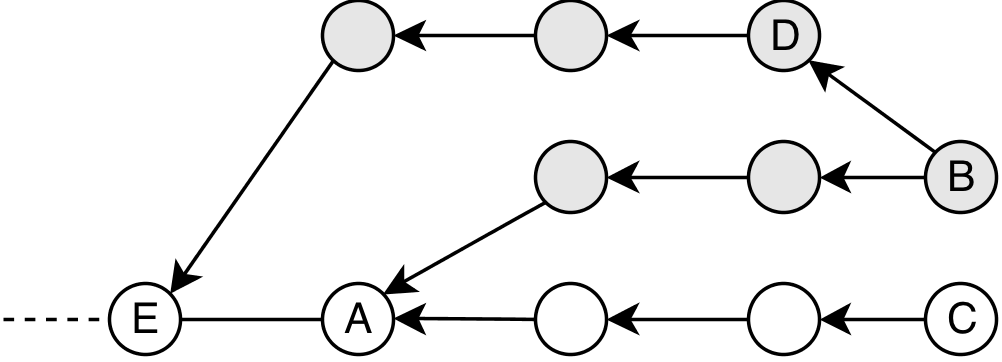
\includegraphics[width=0.6\textwidth]{img/new-commits}
  \caption{Commit difference between branches B and C and A being the last synchronized commit.}
  \label{fig:histo.new-commits}
\end{figure}

We want to ensure that if `commitA' is not part of the history, the entire history of `commitB' is returned.
`getCommonAncestor()' therefore has to return the root of the history if no common ancestor is found.
This is the reason for the exit condition on line 19 where commitB has reached the root of the history.

\subsection{Application Data Change Detection}

Having extracted the list of commits that need to be propagated we can now trace what data has been changed through these.\\
In section \ref{sec:histo.committing} we explained how each object is stored separately under its cryptographic hash.
Existing objects are never updated in-place - we therefore only have to identify which objects have been added to the store.\\

We identify updated objects on a per-commit basis comparing each commit's state with its ancestors.
Starting at the root object referenced by the commit we recursively difference the hierarchy with the commit's ancestor:

\begin{lstlisting}[caption=Detecting data difference across commits, label=data-difference]

function getDataDifference(rootObjectHash, ancestorRootObjectHash) {
  result = []

  if (rootObjectHash == ancestorRootObjectHash) {
    return result
  }

  result.push(rootObjectHash)

  rootObject = store.read(rootObjectHash)
  ancestorRootObject = store.read(ancestorRootObjectHash)
  rootChildren = rootObject.getChildDictionary()
  ancestorChildren = ancestorRootObject.getChildDictionary()

  childDifference = getDictionaryDifference(ancestorChildren, rootChildren)

  for (each insertedChildHash in childDifference.inserts) {
    insertedChildAllChildren = getChildrenRecursive(insertedChildHash)
    result.push(insertedChildHash)
    result.concat(insertedChildsAllChildren)
  }

  for (each update in childDifference.updates) {
    updatedChildHash = update.new
    updatedAncestorChildHash = update.ancestor
    childResult = getDataDifference(updatedChildHash, updatedAncestorChildHash)
    result.concat(childResult)
  }

  return result
}

\end{lstlisting}

In our scenario the children correspond to embedded instances as we defined them in section \ref{sec:histo.hierarchy}.
While in our data model we differentiate between instances belonging to certain attributes this is not relevant for the data difference algorithm.
We simply flatten the embedded child instances across all attributes to a single dictionary of children.\\
The dictionary difference algorithm that is used in the `getDictionaryDifference()' call is explained in section \ref{sec:histo.merging.diff}.
In the context of the section it is used for merging but we can re-use the algorithm for our purpose here.\\
Through the combination of the commit and data difference algorithms we now have the tools to implement the update detection and update propagation steps of our synchronization protocol as described in section \ref{sec:histo.protocol}.
